
\chapter{Demonstration}
%%%%%%%%%%
\label{chap:demo}

\acrshort{DSR} demands a utilization of the artifact in at least one use case. In reference modeling, the model's purpose in practice is its application on a company in the form of an application model. 

Arvato, introduced in chapter \ref{chap:case}, is subject to the instantiation of the domain reference model to a provider model (\cf \Fig \ref{fig:modellevels}). The provider model intentionally embodies individual characteristics, so that changes to the domain reference model are inevitable. These changes specialize, but do not contradict, research in this thesis. 

Documents and interview transcripts are foundation of the following practical exhibition. The interviewees were asked open questions about their business understanding and the reference model was not used to structure the interview in the first place. Consequently, their statements have to be located in the model. 

	\section{Process Framework}
	
	Following a top-down structure, starting point is the most abstract layer of the model.
	 \Tab \ref{tab:interv} gives an overview about covered aspects in interviews. The interviews cover all processes, except \textsc{Inbound Service} and \textsc{Outbound Service}. For these, results from the process modeling workshop are available. The author was part of the workshop and conducted all interviews. 

\begin{table}[caption={Interviews and Relations to Processes}, label={tab:interv}]
	\centering
	
	\begin{tabular}{p{1cm} p{3.4cm}  p{4cm}  p{5cm} }
		\textbf{Order} & \textbf{Topic} & \textbf{Interviewee}          & \textbf{Relation to Processes}                          \\ \hline \hline
		1                            & Model expectations            & Member of the board                  &                                                                         \\\hline
		2                            & Sales                         & Global sales manager                 & \textsc{Sales}, \textsc{Transition}                                                       \\\hline
		3                            & IT                            & Global IT manager                    & \textsc{Transition}                                                              \\\hline
		4                            & Operations                    & Global operations manager            & \textsc{Quality}, \textsc{People Lifecycle}, \textsc{Operations Management} \\\hline
		5                            & Portfolio \& Solution Design  & Global portfolio manager             & \textsc{Product Development}, \textsc{Portfolio Management}, \textsc{Solution Design }             \\\hline
		6                            & Solution Design \& Consulting & Senior consultant                    & \textsc{Product Development}, \textsc{Portfolio Management}, \textsc{Solution Design}              \\\hline
		7                            & Self-Services     & Global portfolio \& solution manager & \textsc{Self-Services}, \textsc{Solution Design}, \textsc{Knowledge Management}                     \\\hline
		8                            & Account Management            & Key account manager                  & \textsc{Transition}, \textsc{Account Management  }                                                    \\\hline
		9                            & Implementation                & Global sales manager                 & \textsc{Transition}                                                             
	\end{tabular}
\end{table}

	Regarding the overall split into management, client and customer processes, interviewees conveyed that Arvato divides into global and local responsibilities.
	Interview partners in a global role reflect on differences between country organizations, while a local view is taken within a country organization. Managerial processes were found on a global level. Client and customer processes were discussed from a global and local perspective. 
	
	Product orientation of Arvato and its competitors was affirmed in the interviews. Compatibility between the understanding of portfolio, products and solutions in this work and at Arvato is given.
	
	 The provider model is shown in \Fig \ref{fig:arvatofram} and detailed in the remainder of this chapter.
	
\begin{figure}[caption={Arvato Framework}, label={fig:arvatofram}]
	{	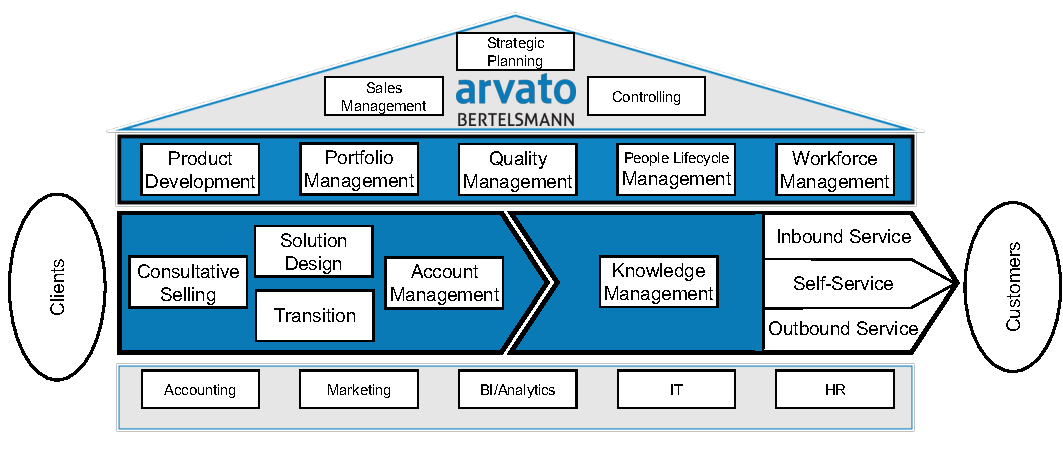
\includegraphics[width=.98\textwidth]{figures/frameworkA.pdf} 
	}
\end{figure}


	%%%%%%%%%%
	%%%%%%%%%%
	
	\section{Customer Processes}
	
	Practical evidence for the four processes in this area is seen in the interview regarding self-services (relating to \textsc{Self-Services} and \textsc{Knowledge Management}) and the process modeling workshop (relating to \textsc{Inbound} and \textsc{Outbound Services}).
	
		\subsubsection{Inbound \& Outbound Services}
	Building on the workshop at one location covering multiple clients in tourism and financial services, a clear picture about operations in a contact center was captured. 
	As voice, video, email, chat, twitter and facebook interactions were covered, all four channel types introduced in this thesis (voice, mail, direct messenger, social) have been explored. As participating managers shared their perception on inter-personal service interactions across client businesses located at their site, an abstraction from client-specific details can be assumed. The outcomes of the workshop were generalized to approximate the detail level within the process reference model. \textsc{Inbound Service} and \textsc{Outbound Service}, as modeled in \ref{pr:inb}, \ref{pr:out}, cover more details than found in the workshop outcomes: As analytical support was very limited and no central customer database was existing, several reference model process steps have to be seen as optional in an application on this client case. However, as one specific client business is seen as a client model instead of a provider model, the supported optionality of process steps in icebricks protects integrity. An omission of these optional steps in the client model can be realized.
	
	\subsubsection{Self-Services \& Knowledge Management}
	The interviewee saw customer needs in center of \textsc{Self-Service}, which is aligned to the reference process. However, it was admitted that difficulties arise in a process representation, because the diversity of self-service utilization implies different procedures. The representation in this work corresponds to the \textit{maintenance} phase of self-service technologies, which follows the \textit{project} phase according to the interviewee. The latter describes the implementation of a self-service and can be seen as part of \textsc{Solution Design} and \textsc{Transition} in the reference model. The maintenance phase especially consists of back-end processes, that are covered in \textsc{Knowledge Management}. Explicitly the creation and maintenance of content \wrt customer needs was mentioned in this regard. The proposed split to case-, transaction-, and customer-related knowledge  in the reference process is hence supported regarding the \textit{case} dimension. In addition, customer- and transaction-related knowledge was deemed important in inter-personal services. 
	
	\textsc{Self-Service} is modeled from a system perspective, therefore it must adequately represent used self-service systems from Arvato. Chat bots and semantic search can be named to give a channel-integrated and stand-alone example. While a chat bot must perform the reference process for every message in a conversion, a single passing through the steps can represent semantic search. The abstract \textit{customer need}  object enables the demonstration of both applications in the reference process.   

	Regarding terminology, the notion \textit{next best action} shall be used instead of \textit{resolution} for Arvato. 
	%%%%%%%%%%
	%%%%%%%%%%
	\section{Client Processes}
	Interviews 2,3,9 and 8 relate to the different stages of the outsourcing lifecycle. \textsc{Solution Design} was part of interview 5,6 and 7 of \Tab \ref{tab:interv}.
	
	While the general structure of the client processes is seen as applicable to Arvato, a customization is applied to emphasize strategic priorities of the organization. \textsc{Sales} is renamed \textsc{Consultative Selling}, as it differentiates Arvato from competitors. 
	
	\subsubsection{Consultative Selling}
	
	This approach puts more emphasis on proactive activities in pre-sales, which is seen in the first two detail processes (\textit{identify prospect} and \textit{approach prospect}). The following steps conform to \textit{Bid Management} at Arvato, where a detailed process description is existing that can be matched with the reference detail processes. For the provider model, this documentation is used to specify process building blocks (\cf Appendix \ref{app:salesbb}). 	The importance of the  \acrshort{RFP} is stressed by Arvato, which conforms to the reference model. \textit{Perform due diligence}, \textit{negotiate contract} and \textit{create commercial deal} are not explicitly listed as parallel processes, but covered in the documentation. %Contract creation is seen as part of \textit{Contract Management} at Arvato. 
	
	\subsubsection{Transition}
	
	Implementation or transition are used to describe the phase between a signed contract and start of final service delivery. As discussed in \ref{pr:tra}, it was affirmed that the process starts during contract finalization, which also supports a separate process on framework level.  A transition plan was not explicitly mentioned, but it can be assumed that information is compiled in one or more documents that structure the transition project. 
	
	The interviewee stated that the most important question in this process is about the location of knowledge and documentation, which is captured in the \textit{transfer business, people, process, technology} detail processes. The proposal to segment into people, process and technology was consented. In addition, the initial recruiting and training of \acrshort{CSR}s was named, which is part of \textsc{People Lifecycle Management} in the reference model. 
	
	While \acrshort{PMO} and \acrshort{TMO} phase were not explicitly mentioned, their concepts were expressed during the interview. It was stated that it is recommended to start the transfer without further changes (corresponding \acrshort{PMO}). After this phase, optimization of status-quo (\ie, \acrshort{TMO}) can be initiated. 
	
	\subsubsection{Account Management}
	 \textsc{Sales} and \textsc{Account Management} can be linked together in country organizations inside Arvato. This view was taken in interview 8 and therefore a scoping of process boundaries was necessary. Starting point of \textsc{Account Management} was seen at the latest with signing of the contract and therefore the process is effective during \textsc{Transition}. Constituents of the reference process were named in the interview, namely service performance monitoring, contract management and especially relationship management. The interviewee emphasized change management, that is not explicitly modeled as a detail process, but captured in \textit{manage disputes}, \textit{propose innovation} and \textit{renegotiate contract}. As a lifecycle analogy was stated, \textit{end contract} is a suitable last detail process. 
          
   	\subsubsection{Solution Design}
	\textsc{Solution Design} as a process in the reference model corresponds to the field of action of a same-named \textit{organizational unit} within the German Arvato organization. This unit also consults in pre-sales activities, that are not part of this process. 
	
	The interviewee stated that starting point during pre-sales is the \textit{identification of potentials for improvement}, from which service requirements are derived. Then, with help of the product portfolio, a client-specific solution is created. The following development is conducted by IT. While the transformation towards a product-oriented organization is aimed, it was admitted that this is work in progress. 
	
	Abstracting from organizational structure, one can state that the described process at Arvato is covered in parts of \textsc{Consultative Selling} and \textsc{Solution Design}. As intended by separate modeling of the \textsc{Solution Design} process, it supports during sales activities. The following justifies the split between consulting and design. 
	
	The reference process starts with \textit{process service challenge}, that assumes challenges are identified in \textsc{Consultative Selling} and used in \textsc{Solution Design} to identify the problem. The specification of these challenges in a proactive or reactive manner is seen as core part of consultative business and consequently must be located as part of \textsc{Consultative Selling}. In turn, designing is focus of \textsc{Solution Design}. 
	
	\section{Management Processes}
	Aim of demonstrating these processes must be their applicability across client businesses, which is embodied through a global pendant at Arvato. Product- and portfolio-related activities fall under responsibility of global \textit{Portfolio \& Solution Design}. It is per definition task of \textit{Operations} to handle service delivery on an executing level. To capture ambitions within Arvato to align operational business across the organization, a global operations initiative was founded to create a framework for harmonization and standardization. Hence, the \textsc{Quality Management}, \textsc{People Lifecycle Management} and \textsc{Operations Management} reference processes must cover their sphere of activity. Available process descriptions were used to enhance detail level. 
	
	Interviews 4 and 5 were subject to processes that strive for alignment across the organization. In addition, documents regarding the available global operations framework are considered for demonstration. A comparison in terms of terminology unveiled that \textsc{Workforce Management} is used instead of \textsc{Operations Management} at Arvato. To foster understanding of the framework, the process is renamed.
	
	%%%%%%%%%%
	\subsubsection{Product Development \& Portfolio Management}
	
	Arvato is in the process of establishing a product orientation. Building a common mindset in differentiating products and solutions is one challenge. Because of this, a separated product development process, isolated from \textsc{Solution Design}, is not defined. However, it was stated that products must be conceptual, derived from market instead of client requirements and the basis for client-specific solution. Essentially, this constitutes the existence of a separate \textsc{Product Development} process as specified in the reference model. 
	
	Awareness for \textsc{Portfolio Management} is existing at Arvato and justified in aspirations to standardize and harmonize \acrshort{CRM} platforms. Furthermore increased transparency was named as one driver, that signifies two views that are taken on the portfolio at Arvato. The \textit{Sales Portfolio} conveys an external view on the products that is communicated towards clients, while the \textit{Delivery Portfolio} links products to internal components and splits these into people, process and platform components. 
	
	A comparison to the reference model demonstrates similarities. With platform components being understood as technology components, the reference model's portfolio structure is a suitable representation of practice at Arvato. 
	In addition to components that relate to one or multiple products, the need of having additional documentation and marketing material was stated, so that a use in \textsc{Solution Design} and \textsc{Consultative Selling} is enabled. 
	
	\subsubsection{Quality Management}
	Quality is deliberately defined widely within this process, so that individual \acrshort{CSR} and overall service delivery performance is covered. The global operations framework lists Staff Performance Management, Quality Management and Client Communication as components, that can be put into relation to the \textsc{Quality Management} reference process. While client communication is part of \textsc{Account Management}, the idea of constant improvement of service delivery is conveyed within \textsc{Quality Management} as well as the reporting function. 
	
	 
	\subsubsection{People Lifecycle Management}
	People, Employee or Agent Lifecycle Management is seen as an integral constituent of HR management in the organization. The mission of People Lifecycle Management at Arvato is the creation of \enquote{a professional environment that attracts the right talent, where performance is rewarded through empowerment, continuous learning and personal development – enabling people to achieve their potential while efficiently and effectively surpassing customer expectations.} However, a detailed process representation was not found. 
	
	To demonstrate the applicability of \textsc{People Lifecycle Management} to the organizational context, lifecycle constituents at Arvato can be compared with reference detail processes. The interviewee mentioned \textit{selecting}, \textit{hiring} and \textit{onboarding} as initial phases, that correspond to the first three steps of the reference process. The following \textit{career path} within Arvato describes the following detail processes and the employee's \textit{attrition} conforms to \textit{let go employee}.
	
	\subsubsection{Workforce Management}
	
	A detailed process description for \textit{Workforce Management} illustrates its similarities to \textsc{Operations Management}. The process at Arvato is composed of \textit{Forecasting} (1), \textit{Capacity Planning} (2), \textit{Scheduling} (3), \textit{Real Time Management} (4) and \textit{Reporting} (5). The first four steps can clearly be mapped to the reference detail processes. The process in the application model is adjusted in form of an additional \textit{perform reporting} detail process and specified process building blocks based on Arvato documents in Appendix \ref{app:wfm}.
	
	
	%\enquote{Putting the right people, with the right skills, in the right place, at the right time, to balance our client expectations, optimize internal efficiencies, while considering our unique employee requirements.}
	
%	plan, execute, control, analyze
%	forecasting, cap plan, scheduling, rtm, analyze
%	external, internal, 

	
	
